\newpage
\section{Action abstractions}


\epigraph{
A green leaf, is too far, out of reach,
What you want, is in front, take the steps.

You move your first leg up You move your second leg left ... You move your eleventh leg up You move your twelfth leg right

Many legs burden the act,
Unless coordinated in abstract.

The abstract words in this new language,
Must be as few as we can manage.

"left", "right", "forward", "backward"

This time, the act is rather brief,
"forward", to reach the tasty leaf.
}{\textit{The writer and poet: Alex Telfar}}


Action abstraction is possibly the least explored type of abstraction.
There exists a lot of work seeking state abstraction (refs), and heirarchical (temporal) abstraction (refs)
but, this has only recently been some work ...

\subsection{Interfaces}

The intution is.
People can generalise / adapt between different action spaces.

\begin{itemize}
\tightlist
\item
  Might be teleported to a new environment? (new state space, same
  action space)
\item
  Might have to drive a new vehicle (same state space, new action space)
\end{itemize}


Utility?
- Adapt to broken limbs
- To new ?

% ref sergey levine meta adaptation limb paper!?

\begin{figure}
\centering
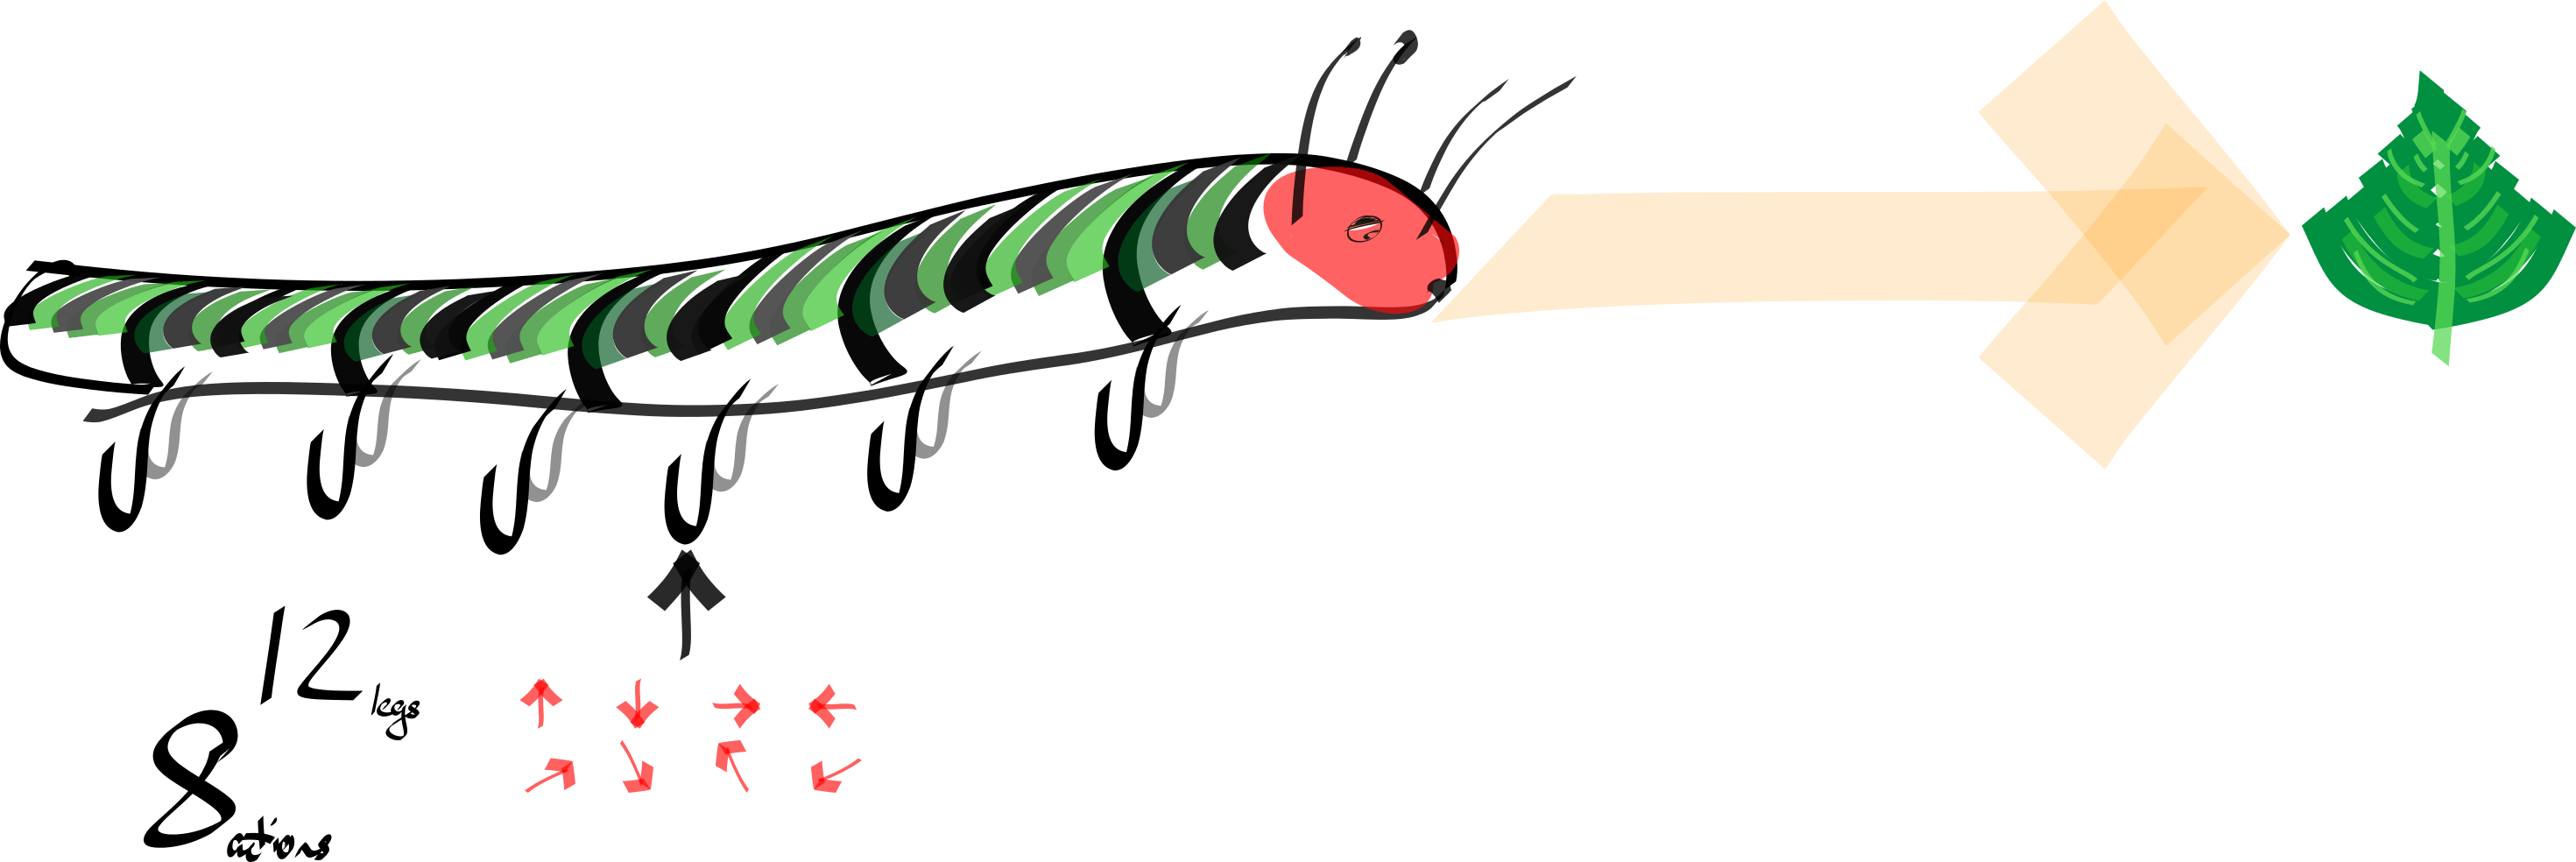
\includegraphics[width=\textwidth,height=0.25\textheight]{../../pictures/drawings/hungry-caterpillar.png}
\caption{Consider a hungry caterpillar. It wants to move towards the leaf. But this is a complicated task! Move your 3rd leg up, your 7th leg down, 11th lag slignly forward, etc...}
\end{figure}


\begin{figure}
\centering
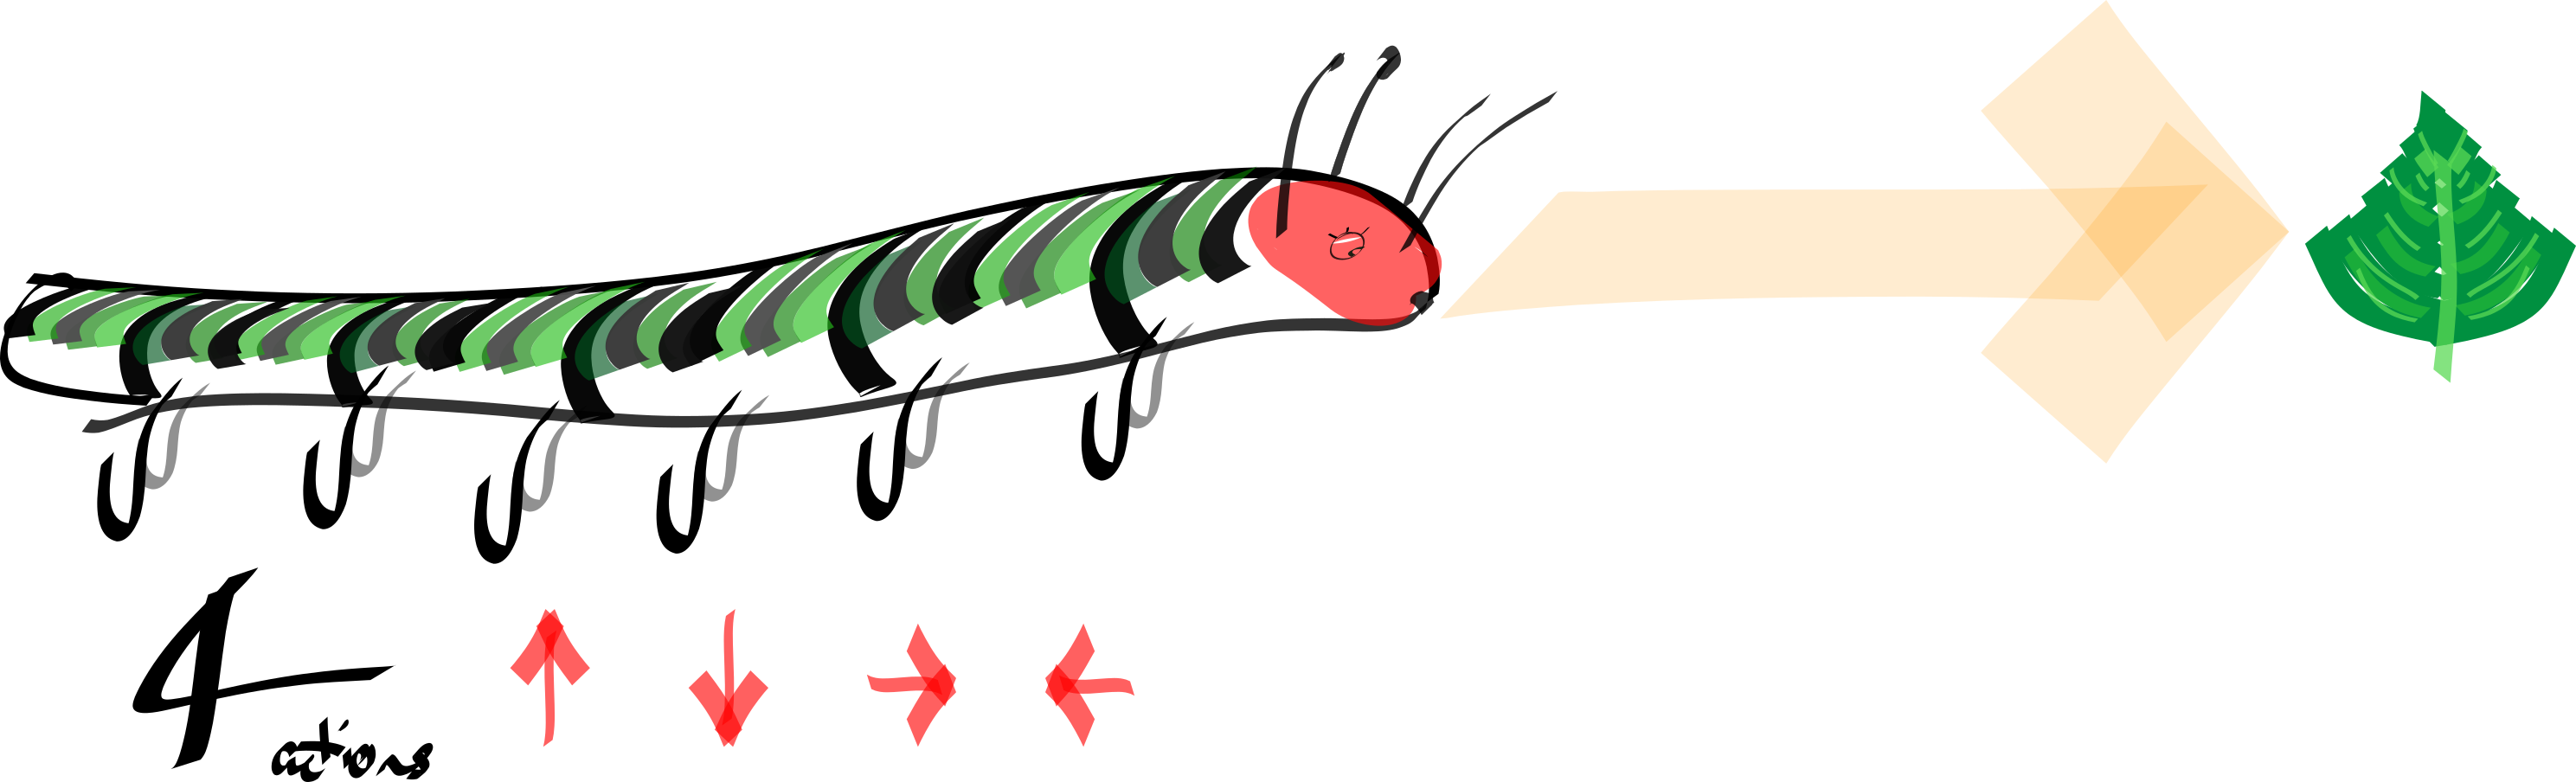
\includegraphics[width=\textwidth,height=0.25\textheight]{../../pictures/drawings/full-caterpillar.png}
\caption{But, what if it could specify actions in another way? Rather than specifying leg movements, it could pick a direction to move, which would specify a program of leg movements.}
\end{figure}


% \begin{figure}
% \centering
% \includegraphics[width=0.5\textwidth,height=0.5\textheight]{../../pictures/figures/discrete-interface.png}
% \caption{The optimisation dynamics of value iteration versus parameterised value iteration.}
% \end{figure}


\subsection{Related work}

\cite{Nagabandi2019}
